\documentclass[11pt]{article}

\usepackage[margin=1in]{geometry}
\usepackage{amsmath,amssymb,amsthm}
\usepackage{mathtools}
\usepackage{tikz}
\usetikzlibrary{arrows.meta,calc,positioning}
\usepackage{enumitem}
\usepackage{hyperref}
\usepackage{microtype}
\usepackage{titlesec}
\usepackage{fancyhdr}

\hypersetup{colorlinks=true,linkcolor=black,urlcolor=blue,citecolor=black}
\setcounter{tocdepth}{2}
\numberwithin{equation}{section}

\titleformat{\section}{\large\bfseries}{\thesection.}{0.6em}{}
\titleformat{\subsection}{\normalsize\bfseries}{\thesubsection}{0.5em}{}

\pagestyle{fancy}
\fancyhf{}
\fancyhead[L]{\small Classical Mechanics notes}
\fancyhead[R]{\small Susskind, Theoretical Minimum, Fall 2011}
\fancyfoot[C]{\thepage}
\renewcommand{\headrulewidth}{0.3pt}

\newcommand{\qdot}{\dot{q}}
\newcommand{\pdot}{\dot{p}}
\newcommand{\ddt}{\frac{d}{dt}}
\newcommand{\pd}[2]{\frac{\partial #1}{\partial #2}}
\newcommand{\vect}[1]{\mathbf{#1}}
\newcommand{\epsijk}{\varepsilon_{ijk}}

\title{Classical Mechanics\\[0.4em]
\large Notes on Leonard Susskind, \emph{The Theoretical Minimum}\\
Stanford Continuing Studies, Fall 2011}
\author{}
\date{}

\begin{document}
\maketitle
\vspace{-2em}
\begin{center}
\small Unofficial study notes from the ten lectures at\\
\url{https://theoreticalminimum.com/courses/classical-mechanics/2011/fall}\\[0.3em]
Not a transcript. Not a substitute for the lectures or the book.
\end{center}

\tableofcontents
\newpage

%----------------------------------------------------------------------
\section{Lecture 1. State diagrams and the nature of physical laws}

A physical law is a rule that takes the present state of a system and returns the next one. Before $F=ma$, the question is which rules are allowed: which ones let you predict the future and reconstruct the past. That filter is the minus-first law. On a finite state space, the legal rules are unions of cycles, and the name of the cycle you occupy is a conserved quantity.

\subsection{States and dynamical laws}

A system has a set of possible states. A \emph{dynamical law} assigns to each state a successor.

The coin has two states, $H$ and $T$. A law is a pair of assignments, $H\mapsto{}$something and $T\mapsto{}$something. The die has six states. A particle on a line has a continuum of states; the same language still applies, with the discrete arrow replaced by a map $\mathbb{R}\to\mathbb{R}$ or, once velocities are in the game, a map on a bigger space.

The \emph{configuration} of a system is where it is (heads, or the positions of $N$ particles). The \emph{state} is whatever you must know to run the law. For the coin they coincide. For Newtonian particles they do not: you also need how the configuration is changing. That distinction is Lecture~2. Here the point is only that the law is a map on whatever you have chosen to call the state.

\subsection{Determinism and reversibility}

Classical physics requires two properties of that map.

\begin{itemize}[leftmargin=1.4em]
\item \textbf{Determinism.} From the present state there is exactly one next state. One arrow out of each state. The future is fixed.
\item \textbf{Reversibility.} There is exactly one previous state. One arrow into each state. The past is fixed.
\end{itemize}

Together: every state has exactly one arrow in and one arrow out. Susskind calls this the conservation of information, and sometimes the minus-first law: you always know where you are going and where you came from.

If two arrows enter one state, two distinct pasts become the same present and you cannot tell them apart. Information is lost. If a state has no incoming arrow, nothing in the dynamics ever produces it, so you cannot reverse into it. If a state has two outgoing arrows, the law has not decided the future.

The minus-first law is prior to energy, momentum, and $F=ma$. It is a constraint on the \emph{form} of a law. A proposed rule that collapses many states into one, or that has a sink with no inverse, is not a classical law in this sense, even if you can write a differential equation for it.

\subsection{Cycles are conservation laws}

On a finite set, a map that is one-to-one (and onto) is a permutation, and every permutation decomposes into disjoint cycles.

Examples for the coin.
\begin{itemize}[leftmargin=1.4em]
\item Stay put: $H\to H$, $T\to T$. Two 1-cycles.
\item Always flip: $H\to T$, $T\to H$. One 2-cycle.
\item Both flow to $H$: $H\to H$, $T\to H$. Illegal. $H$ has two arrows in, $T$ has none. From $H$ you cannot recover whether the past was $H$ or $T$.
\end{itemize}

A six-sided die with $n\mapsto n+1\pmod{6}$ is one 6-cycle. A law that swaps $1\leftrightarrow 2$, cycles $3\to 4\to 5\to 3$, and leaves $6$ fixed has three cycles. If you start on one cycle you stay on that cycle forever. The label of the cycle is a conserved quantity: an integer you can read off the state, constant along the motion, that tells you which sector you occupy.

That is the discrete prototype of every conservation law later in the course. Phase space will split into surfaces of constant energy, constant momentum, constant angular momentum. The motion never jumps surfaces, for the same reason the die never jumps cycles: the law has no arrows between them.

\subsection{Infinite configuration spaces}

Unlimited numbers of states are allowed. A particle on the line, state $x\in\mathbb{R}$, with $x\mapsto x+a$ is legal (invertible). $x\mapsto x^3$ on $\mathbb{R}$ is not: three preimages for some points, none for others. $x\mapsto e^x$ misses the negatives.

The same rule: the dynamical law must be a one-to-one map on the state space. Colliding arrows, or arrows that dump a region of states into a lower-dimensional set, are still forbidden. Liouville's theorem (Lecture~7) is this statement for Hamiltonian flow, with ``number of states'' replaced by phase-space volume.

\subsection{Predictability in the world}

Determinism is a property of the law plus the exact state. It does not say that a finite-precision measurement determines the far future. A map can be one-to-one and still stretch nearby states apart (sensitive dependence). Then you can reconstruct the past and predict the future in principle, and still fail in practice. The minus-first law is not a claim about weather forecasts. It is a claim about the arrows.

\subsection{Point particles}

A system of $N$ point particles in 3-space has configuration
\[
(\vect{r}_1,\ldots,\vect{r}_N)
= (x_1,y_1,z_1,\ldots,x_N,y_N,z_N),
\]
$3N$ real numbers. Configuration is not the full state. Newton's law is a second-order equation, so the law also needs the velocities. The state is $6N$ numbers. The space of those states is phase space.

\subsection{Vectors and the dot product}

A displacement is a vector $\vect{r}$. Addition is the parallelogram rule: $\vect{a}+\vect{b}$ is the diagonal of the parallelogram they span. Scalar multiplication stretches (or flips, if the scalar is negative).

The \emph{dot product} is the scalar
\[
\vect{a}\cdot\vect{b} = |\vect{a}|\,|\vect{b}|\cos\theta,
\]
with $\theta$ the angle between them. It is linear in each slot, and $\vect{a}\cdot\vect{a}=|\vect{a}|^2$. Expand $|\vect{a}-\vect{b}|^2$:
\[
|\vect{a}-\vect{b}|^2
= (\vect{a}-\vect{b})\cdot(\vect{a}-\vect{b})
= |\vect{a}|^2 + |\vect{b}|^2 - 2\,\vect{a}\cdot\vect{b}.
\]
That is the law of cosines for the triangle with sides $\vect{a}$, $\vect{b}$, $\vect{a}-\vect{b}$. In an orthonormal basis,
\[
\vect{a}\cdot\vect{b} = a_x b_x + a_y b_y + a_z b_z.
\]
The geometric definition and the component formula agree because $\hat{\vect{e}}_i\cdot\hat{\vect{e}}_j=\delta_{ij}$.

The cross product appears when we need area and angular momentum (Lecture~4) and magnetic force (Lecture~9).

\subsection{Velocity, acceleration, circular motion}

A trajectory is a curve $\vect{r}(t)$. Velocity and acceleration are
\[
\vect{v} = \dot{\vect{r}} = \ddt\vect{r},\qquad
\vect{a} = \dot{\vect{v}} = \ddot{\vect{r}}.
\]
In Cartesian components, $\vect{v}=(\dot x,\dot y,\dot z)$ and likewise for $\vect{a}$. The derivative of a product of vectors follows the usual Leibniz rule, including
\[
\ddt\bigl(|\vect{r}|^2\bigr) = 2\,\vect{r}\cdot\vect{v}.
\]
If the particle stays on a sphere $|\vect{r}|=R$ constant, then $\vect{r}\cdot\vect{v}=0$: velocity is tangent.

Uniform circular motion of radius $R$ and constant speed $v$ is the special case
\[
x = R\cos\omega t,\qquad y = R\sin\omega t,\qquad \omega = \frac{v}{R}.
\]
Differentiate:
\[
\dot x = -R\omega\sin\omega t,\qquad
\dot y = R\omega\cos\omega t,\qquad
|\vect{v}| = R\omega = v,
\]
\[
\ddot x = -R\omega^2\cos\omega t = -\omega^2 x,\qquad
\ddot y = -\omega^2 y.
\]
So $\vect{a}=-\omega^2\vect{r}$, directed toward the center, with magnitude
\[
|\vect{a}| = \omega^2 R = \frac{v^2}{R}.
\]
That centripetal acceleration is not optional: it is what $\ddot{\vect{r}}$ is when $\vect{r}$ goes around a circle at constant speed. If you want circular motion, you need a force $m v^2/R$ inward. If you have no such force, you do not get a circle.

%----------------------------------------------------------------------
\section{Lecture 2. Newton's law, phase space, momentum and energy}

Aristotle's law is a first-order rule for $\vect{r}(t)$: force sets velocity. Newton's law is second order: force sets acceleration, and the default motion is uniform. Because the equation is second order, the state that determines the future is $(\vect{r},\vect{v})$, not $\vect{r}$ alone. That space is phase space. Momentum and energy are the first conserved labels of sectors in that space, coming from the third law and from forces that derive from a potential.

\subsection{Aristotle versus Newton}

Aristotle: force is proportional to velocity. A push is needed to keep moving. That is a decent description of motion in thick air or molasses, where drag quickly balances any applied force and you observe a terminal velocity. It is a first-order law: $\vect{v}=\vect{v}(\vect{F})$. The state would be position alone.

Newton, in empty space: if $\vect{F}=0$, then $\vect{a}=0$. Uniform motion, not rest, is the default. You need a force to \emph{change} velocity, not to maintain it. That is a second-order law for $\vect{r}(t)$.

\subsection{Inertial frames}

Newton's first law (the $\vect{F}=0$ case of the second) does not hold in every coordinate system. An \emph{inertial frame} is one in which a free particle moves with constant velocity. Frames moving at constant velocity relative to an inertial frame are inertial (Galilean relativity): if $\vect{r}'=\vect{r}-\vect{u}t$ with $\vect{u}$ constant, then $\vect{a}'=\vect{a}$. Frames that accelerate or rotate relative to an inertial frame are not inertial. In those coordinates a free particle appears to accelerate. The extra terms are fictitious forces (Lecture~3).

The first law is the test that tells you whether your coordinates are inertial. The second law is then a statement in those coordinates.

\subsection{The second law}

\[
\vect{F} = m\vect{a} = \ddt\vect{p},\qquad \vect{p} = m\vect{v}.
\]
If mass is constant this is $F=ma$. The $dp/dt$ form is the one that survives: it is still correct if $m$ changes, it is the form that pairs with the third law to give momentum conservation, and it is the form Hamilton's equations will reproduce.

$\vect{F}$ is a function of the state, typically of positions (and, for magnetism, of velocities). The law is an ordinary differential equation, not an identity.

\subsection{Why the state is position and velocity}

A second-order equation $\ddot{\vect{r}}=\vect{F}(\vect{r},\vect{v},t)/m$ has a unique solution once you specify $\vect{r}(t_0)$ and $\vect{v}(t_0)$. Position alone is not enough: two particles at the same place with different velocities have different futures. Velocity alone is not enough either.

The state of $N$ particles is $6N$ numbers: three positions and three velocities (or momenta) per particle. That space is \emph{phase space}. A point in phase space, plus the law, determines the whole future and the whole past. That is Newton's version of determinism plus reversibility.

Phase space is not configuration space. Configuration space is $3N$-dimensional. Trajectories that cross in configuration space need not cross in phase space: they can pass through the same $\vect{r}$ with different $\vect{v}$.

\subsection{Time reversal}

Replace $t\to -t$. Then $\vect{v}\to -\vect{v}$ and $\vect{a}\to +\vect{a}$. Newton's law with $\vect{F}=\vect{F}(\vect{r})$ is unchanged: the same force, the same $m\vect{a}$. Running the movie backward is a legal motion. In phase space, time reversal is $(q,p)\to(q,-p)$ together with $t\to -t$.

A force that depends on an odd power of velocity (linear drag, $-\gamma\vect{v}$) flips sign under $t\to -t$ and the law is not reversible. Those laws also fail Liouville (Lecture~7). They describe open systems, with degrees of freedom you have chosen not to track.

\subsection{The three laws, and momentum conservation}

\begin{enumerate}[leftmargin=1.4em]
\item Inertial frames exist: $\vect{F}=0$ implies $\vect{a}=0$.
\item $\vect{F}=\dot{\vect{p}}$.
\item If $A$ pushes $B$ with $\vect{F}_{AB}$, then $B$ pushes $A$ with $\vect{F}_{BA}=-\vect{F}_{AB}$.
\end{enumerate}

The third law is the statement that internal forces cancel in pairs. For an isolated collection of particles,
\[
\ddt\sum_i \vect{p}_i
= \sum_i \vect{F}_i^{\mathrm{ext}}
+ \sum_{i<j}\bigl(\vect{F}_{ij}+\vect{F}_{ji}\bigr)
= \sum_i \vect{F}_i^{\mathrm{ext}}.
\]
If there are no external forces, total momentum $\vect{P}=\sum_i\vect{p}_i$ is constant. In the language of Lecture~1: phase space splits into sectors labeled by $\vect{P}$, and the motion never leaves its sector.

The third law can fail (momentum dumped into a field). When it holds, $\vect{P}$ is conserved because internal arrows cancel, not because we postulated a separate conservation law.

\subsection{Potential energy}

A force on a particle is \emph{conservative} if it is minus the gradient of a function $V(\vect{r})$:
\[
\vect{F} = -\nabla V.
\]
In one dimension, $F(x)=-V'(x)$, and any $F(x)$ is conservative ($V=-\int F\,dx$). In three dimensions the condition is path-independence of work, equivalently
\[
\nabla\times\vect{F}=0
\]
on a simply connected region, in which case $V$ exists.

Why introduce $V$ at all? Because then one combination of $v$ and $x$ is constant, and you get a first integral of the motion without solving the ODE.

Compute, in one dimension:
\[
\ddt\Bigl(\tfrac12 m v^2 + V(x)\Bigr)
= v\bigl(m a + V'(x)\bigr)
= v\bigl(F - F\bigr)
= 0.
\]
The conserved quantity is the energy
\[
E = T + V,\qquad T = \frac{p^2}{2m} = \tfrac12 m v^2.
\]
The kinetic piece is the amount of $E$ stored in motion. The potential piece is the rest, as a function of position. Only the sum is conserved; $T$ and $V$ trade.

For $N$ particles with a potential $V(\vect{r}_1,\ldots,\vect{r}_N)$ that depends only on the positions,
\[
E = \sum_i \frac{p_i^2}{2m_i} + V
\]
is conserved when $V$ has no explicit time dependence:
\begin{align*}
\dot E
&= \sum_i \vect{v}_i\cdot(m_i\vect{a}_i)
+ \sum_i \vect{v}_i\cdot\nabla_i V
= \sum_i \vect{v}_i\cdot\bigl(\vect{F}_i + \nabla_i V\bigr)
= 0.
\end{align*}
Pairwise potentials $V_{ij}(|\vect{r}_i-\vect{r}_j|)$ give internal forces that automatically satisfy the third law, so $\vect{P}$ and $E$ are both conserved for an isolated system.

A time-dependent $V(\vect{r},t)$ (a piston you shove by hand) injects or removes energy. The derivation used $\partial V/\partial t=0$.

\subsection{Harmonic oscillator}

Near a minimum of any smooth $V(x)$,
\[
V(x) = V(x_0) + \tfrac12 V''(x_0)\,(x-x_0)^2 + \cdots,
\]
with $V''(x_0)>0$. Hooke's law is that quadratic piece: $F=-kx$ with $k=V''(x_0)$, and $V=\tfrac12 k x^2$ after shifting the origin. Every small oscillation is a harmonic oscillator. That is why the example is worth doing once, carefully.

The equation is
\[
\ddot{x} + \omega^2 x = 0,\qquad \omega = \sqrt{\frac{k}{m}}.
\]
General solution: $x(t)=A\cos(\omega t+\phi)$, with $A$ and $\phi$ fixed by $(x(0),\dot x(0))$. Energy
\[
E = \frac{p^2}{2m} + \tfrac12 k x^2
\]
is constant. In the $(x,p)$ plane the level set $E=\mathrm{const}$ is an ellipse
\[
\frac{x^2}{2E/k} + \frac{p^2}{2mE} = 1.
\]
The motion runs around that ellipse. Frequency $\omega$ is independent of amplitude: a property of the quadratic potential, not of oscillators in general. The phase-space picture returns with Hamilton's equations in Lecture~6.

%----------------------------------------------------------------------
\section{Lecture 3. Lagrangian, least action, Euler-Lagrange equations}

Newton's law is written in Cartesian coordinates in an inertial frame. Change coordinates (polar, rotating, constrained to a surface) and you must recompute every component of $\vect{a}$ by hand. The Lagrangian formulation is the same physics, written so that you specify $T$ and $V$ in whatever coordinates you have, and the equations come out automatically. The object that makes this work is the action, a number attached to a whole path. The true path is a stationary point of that number.

\subsection{Stationary points of a function}

If $f(x)$ is smooth, a necessary condition for a local min or max at $x_0$ is $f'(x_0)=0$. The same condition holds at a saddle. ``Stationary'' means the first-order change vanishes: $f(x_0+\varepsilon)=f(x_0)+O(\varepsilon^2)$.

The action principle is that statement, with $x$ replaced by a path $q(t)$ and $f$ replaced by a functional $A[q]$.

\subsection{Paths and the action}

Fix endpoints $q(t_1)=q_1$, $q(t_2)=q_2$. A \emph{path} is any smooth function $q(t)$ connecting them. The \emph{action} of a path is
\[
A[q] = \int_{t_1}^{t_2} L\bigl(q(t),\qdot(t),t\bigr)\,dt.
\]
$L$ is the Lagrangian, a function of position, velocity, and maybe time. For ordinary particles in a potential,
\begin{equation}
\label{eq:LTV}
L = T - V
= \sum_i \tfrac12 m_i \dot{\vect{r}}_i^2 - V(\vect{r}_1,\ldots,\vect{r}_N).
\end{equation}
$T-V$, not $T+V$. That minus sign is the choice that will reproduce $F=-V'$. Using $T+V$ would flip the force.

The \emph{principle of stationary action}: the true trajectory is a stationary point of $A$ among nearby paths with the same endpoints. $\delta A=0$. ``Least action'' is the historical name. The condition is that the first variation vanishes. For short times $A$ is often a minimum; in general it can be a saddle. What the physics uses is $\delta A=0$.

\begin{figure}[ht]
\centering
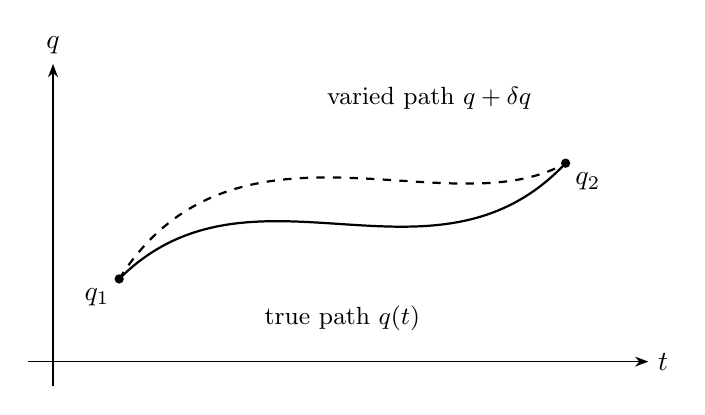
\begin{tikzpicture}[>=Stealth, scale=1.05]
  \draw[->] (-0.3,0) -- (7.2,0) node[right] {$t$};
  \draw[->] (0,-0.3) -- (0,3.6) node[above] {$q$};
  \fill (0.8,1.0) circle (1.6pt) node[below left] {$q_1$};
  \fill (6.2,2.4) circle (1.6pt) node[below right] {$q_2$};
  \draw[thick] (0.8,1.0) .. controls (2.4,2.6) and (4.6,0.7) .. (6.2,2.4);
  \draw[thick, dashed] (0.8,1.0) .. controls (2.2,3.2) and (4.8,1.6) .. (6.2,2.4);
  \node at (3.5,0.52) {\small true path $q(t)$};
  \node at (4.55,3.18) {\small varied path $q+\delta q$};
\end{tikzpicture}
\caption{Stationary action. The endpoints are held fixed, so $\delta q(t_1)=\delta q(t_2)=0$. Among those paths, the true $q(t)$ is the one for which a first-order wiggle does not change $A$. The dashed curve is a competitor, not a second solution.}
\end{figure}

\subsection{Calculus of variations}

Let $q(t)\to q(t)+\varepsilon\,\eta(t)$ with $\eta(t_1)=\eta(t_2)=0$, $\varepsilon$ small. Then
\[
\delta A
= \varepsilon\int_{t_1}^{t_2}\Bigl(
\pd{L}{q}\eta + \pd{L}{\qdot}\dot\eta\Bigr)dt
+ O(\varepsilon^2).
\]
Integrate the second term by parts:
\[
\int_{t_1}^{t_2}\pd{L}{\qdot}\dot\eta\,dt
= \Bigl[\pd{L}{\qdot}\eta\Bigr]_{t_1}^{t_2}
- \int_{t_1}^{t_2}\eta\,\ddt\pd{L}{\qdot}\,dt.
\]
The boundary term dies because $\eta$ vanishes at the endpoints. So
\[
\delta A = \varepsilon\int_{t_1}^{t_2}\eta\Bigl(
\pd{L}{q} - \ddt\pd{L}{\qdot}\Bigr)dt.
\]
If $\delta A=0$ for every such $\eta$, the integrand coefficient must vanish:
\begin{equation}
\label{eq:EL}
\ddt\pd{L}{\qdot} = \pd{L}{q}.
\end{equation}
That is the Euler-Lagrange equation. One copy per coordinate $q_i$.

The same calculation in several variables gives
\[
\ddt\pd{L}{\qdot_i} = \pd{L}{q_i},\qquad i=1,\ldots,n.
\]
No assumption that the $q_i$ are Cartesian. That is the whole point.

\subsection{Two warmups: Fermat and the catenary}

These are stationary-integral problems that are not yet $L=T-V$. They show that the calculus is older than Lagrange, and that ``the path that stationarizes an integral'' is a general machine.

\textbf{Fermat.} Light takes a path of stationary time. Two media, speeds $c_1$ and $c_2$, flat interface. A ray from $(0,h_1)$ in medium~1 to $(a,-h_2)$ in medium~2, hitting the interface at $x$. Travel time
\[
t(x) = \frac{1}{c_1}\sqrt{x^2+h_1^2} + \frac{1}{c_2}\sqrt{(a-x)^2+h_2^2}.
\]
Stationarity, $t'(x)=0$:
\[
\frac{1}{c_1}\frac{x}{\sqrt{x^2+h_1^2}}
= \frac{1}{c_2}\frac{a-x}{\sqrt{(a-x)^2+h_2^2}},
\]
which is
\[
\frac{\sin\theta_1}{c_1} = \frac{\sin\theta_2}{c_2}
\]
($\theta$ measured from the normal). Same calculus as $\delta A=0$, with $L$ replaced by $1/c$ along the path. Snell's law is a stationarity condition, not a separate optical axiom.

\textbf{Catenary.} A hanging chain of fixed length $\ell$ and uniform $\rho$ minimizes potential energy $\rho g\int y\,ds$. With $ds=\sqrt{1+y'^2}\,dx$ and the constraint $\int ds=\ell$, the integrand (Lagrange multiplier $\lambda$ for the length) is
\[
f(y,y') = (y+\lambda)\sqrt{1+y'^2}.
\]
No explicit $x$, so the Beltrami identity $f-y'\,\partial f/\partial y'=\mathrm{const}$ applies. It reduces to
\[
y+\lambda = a\sqrt{1+y'^2},
\]
whose solution is a catenary,
\[
y = a\cosh\Bigl(\frac{x-x_0}{a}\Bigr) - \lambda.
\]
Again a stationary-integral problem, now with a constraint. Mechanical action is the same idea with $L=T-V$ and time as the parameter.

\subsection{Recovering Newton}

One particle, $L=\tfrac12 m\dot x^2-V(x)$. Then
\[
\pd{L}{\dot x} = m\dot x,\qquad
\pd{L}{x} = -V'(x),
\]
so \eqref{eq:EL} is $m\ddot x=-V'(x)$. Same as $F=ma$. For $N$ particles with \eqref{eq:LTV}, Euler-Lagrange in each Cartesian coordinate is $m_i\ddot{\vect{r}}_i=-\nabla_i V$.

The minus in $T-V$ is forced by this match: $\partial L/\partial x$ must be the force, and the force is $-\partial V/\partial x$.

\subsection{Why keep the Lagrangian}

Three reasons, all practical.
\begin{enumerate}[leftmargin=1.4em]
\item \textbf{Arbitrary coordinates.} Write $T$ and $V$ in whatever $q_i$ you like. The form of \eqref{eq:EL} does not change. You never recompute $\vect{a}$ in the new basis by hand.
\item \textbf{Constraints.} If the system is stuck to a surface, use coordinates on that surface. $T$ is the kinetic energy of the allowed motion. The constraint forces never appear.
\item \textbf{The rest of physics.} Field theory and path-integral quantum mechanics are written as stationary action. Learning $L$ here is the cheap version of that move.
\end{enumerate}

A total time derivative can always be added to $L$:
\[
L \to L + \ddt F(q,t)
\]
changes $A$ by $F(q_2,t_2)-F(q_1,t_1)$, which is fixed when the endpoints are fixed, so $\delta A$ is unchanged. Two Lagrangians that differ by $\dot F$ are the same physics. Gauge transformations (Lecture~9) are an instance.

\subsection{Coordinate changes: polar}

Two-dimensional motion, polar coordinates:
\[
x=r\cos\theta,\qquad y=r\sin\theta.
\]
Then $\dot x=\dot r\cos\theta-r\dot\theta\sin\theta$, $\dot y=\dot r\sin\theta+r\dot\theta\cos\theta$, and
\[
T = \tfrac12 m(\dot x^2+\dot y^2) = \tfrac12 m\bigl(\dot r^2 + r^2\dot\theta^2\bigr).
\]
If $V=V(r)$ only,
\[
L = \tfrac12 m\dot r^2 + \tfrac12 m r^2\dot\theta^2 - V(r).
\]
Euler-Lagrange in $r$:
\[
\ddt(m\dot r) = m r\dot\theta^2 - V'(r),
\]
or
\[
m\bigl(\ddot r - r\dot\theta^2\bigr) = -V'(r).
\]
The $r\dot\theta^2$ term is centripetal acceleration, produced automatically by writing $T$ in polar coordinates. You did not put it in by hand.

\subsection{Cyclic coordinates and angular momentum}

A coordinate that does not appear in $L$ (only its velocity does) is \emph{cyclic}. For $\theta$ above, $\partial L/\partial\theta=0$, so Euler-Lagrange says
\[
\ddt\pd{L}{\dot\theta} = 0
\implies
p_\theta := \pd{L}{\dot\theta} = m r^2\dot\theta
\]
is constant. That is angular momentum about the origin, $L_z=x p_y-y p_x=m r^2\dot\theta$.

A cyclic coordinate is a symmetry $\theta\to\theta+\varepsilon$ sitting in the notation: $L$ does not care about the origin of $\theta$. Lecture~4 turns that observation into Noether's theorem. The reason $p_\theta$ is conserved is that the potential has no preferred angle.

\subsection{Rotating frames and fictitious forces}

Write $L$ in a frame that rotates at constant $\omega$ about $\hat{\vect{z}}$ relative to an inertial frame. If $(x,y,z)$ are the rotating-frame Cartesian coordinates of the particle, the inertial coordinates are
\[
x_{\mathrm{in}} = x\cos\omega t - y\sin\omega t,\qquad
y_{\mathrm{in}} = x\sin\omega t + y\cos\omega t,\qquad
z_{\mathrm{in}}=z.
\]
A short computation gives
\[
\dot x_{\mathrm{in}}^2 + \dot y_{\mathrm{in}}^2
= (\dot x-\omega y)^2 + (\dot y+\omega x)^2,
\]
so
\[
L = \tfrac12 m\bigl[(\dot x-\omega y)^2 + (\dot y+\omega x)^2 + \dot z^2\bigr] - V.
\]
Equivalent vector form: $\vect{v}_{\mathrm{in}}=\vect{v}+\vect{\omega}\times\vect{r}$ with $\vect{v}=(\dot x,\dot y,\dot z)$, and
\[
L = \tfrac12 m\bigl|\vect{v}+\vect{\omega}\times\vect{r}\bigr|^2 - V
= \tfrac12 m\vect{v}^2 + m\vect{v}\cdot(\vect{\omega}\times\vect{r}) + \tfrac12 m|\vect{\omega}\times\vect{r}|^2 - V.
\]
The middle term is linear in velocity. The last extra term is quadratic in $\omega$ and looks like a negative potential.

Euler-Lagrange in $x$:
\[
\pd{L}{\dot x} = m(\dot x-\omega y),\qquad
\ddt\pd{L}{\dot x} = m(\ddot x-\omega\dot y),
\]
\[
\pd{L}{x} = m\omega(\dot y+\omega x) - \pd{V}{x}.
\]
So
\[
m\ddot x = 2m\omega\dot y + m\omega^2 x - \pd{V}{x},
\]
and similarly
\[
m\ddot y = -2m\omega\dot x + m\omega^2 y - \pd{V}{y}.
\]
In vector form,
\[
m\vect{a}
= -\nabla V
- 2m\,\vect{\omega}\times\vect{v}
- m\,\vect{\omega}\times(\vect{\omega}\times\vect{r}).
\]
The second term on the right is the Coriolis force, the third is the centrifugal force (outward: $-\vect{\omega}\times(\vect{\omega}\times\vect{r})$ points away from the axis). They are not new interactions. They are what Newton's law looks like after a time-dependent coordinate change. The Lagrangian did the change of coordinates for you.

The Coriolis term is linear in $\vect{v}$, like the magnetic force. That analogy is Lecture~9: $q\,\vect{v}\cdot\vect{A}$ in $L$ plays the same structural role as $m\vect{v}\cdot(\vect{\omega}\times\vect{r})$.

%----------------------------------------------------------------------
\section{Lecture 4. Symmetry and conservation laws}

A conservation law is a first integral: a function of the state that is constant along the motion. You can hunt for them by luck, or you can read them off symmetries of $L$. Noether's theorem is that dictionary: a continuous symmetry produces a conserved charge. Momentum, angular momentum, and (next lecture) energy are the charges for translation, rotation, and time translation.

\subsection{What counts as a symmetry of the Lagrangian}

A \emph{continuous symmetry} is a family of maps on the coordinates, parameterized by a small $\varepsilon$, that leaves $L$ unchanged, or changes it by a total time derivative (which does not affect the equations). Discrete maps (parity, $x\to -x$) can leave $L$ invariant too. They do not give a Noether charge, because there is no infinitesimal $\varepsilon$ to expand in.

If $L$ does not depend on $q_i$, the shift $q_i\to q_i+\varepsilon$ is a symmetry. That is the cyclic-coordinate case, already used. Noether covers symmetries that mix several coordinates (rotations) and symmetries that move the independent variable (time translation).

\subsection{Generalized coordinates and conjugate momenta}

Coordinates $q_i$ need not be Cartesian: angles, distances along a slope, whatever covers the configuration. The \emph{canonical conjugate momentum} to $q_i$ is
\begin{equation}
\label{eq:pdef}
p_i = \pd{L}{\qdot_i}.
\end{equation}
This $p_i$ need not equal $m\dot q_i$. In polar coordinates, $p_\theta=m r^2\dot\theta$. In a magnetic field it will include $q A_i$ (Lecture~10). Euler-Lagrange in this notation is
\[
\dot p_i = \pd{L}{q_i}.
\]
If $q_i$ is cyclic, $\partial L/\partial q_i=0$, so $\dot p_i=0$. Cyclic coordinate if and only if conserved conjugate momentum.

The map $\qdot\mapsto p$ is what the Hamiltonian will invert (Lecture~5). Already here, $p_i$ is the quantity the equations want to conserve when $q_i$ is ignorable.

\subsection{Noether's theorem}

Infinitesimal change of coordinates
\[
q_i \to q_i + \varepsilon\,\eta_i(q),
\]
with $\eta_i$ a specified set of functions (the ``generator''). The first-order change in $L$ is
\[
\delta L
= \varepsilon\sum_i\Bigl(
\pd{L}{q_i}\eta_i + \pd{L}{\qdot_i}\dot\eta_i\Bigr).
\]
On a solution of Euler-Lagrange, $\partial L/\partial q_i=\dot p_i$, so
\[
\delta L
= \varepsilon\sum_i\bigl(\dot p_i\,\eta_i + p_i\dot\eta_i\bigr)
= \varepsilon\,\ddt\Bigl(\sum_i p_i\eta_i\Bigr).
\]
If the transformation is a symmetry in the strict sense $\delta L=0$, then
\begin{equation}
\label{eq:Noether}
Q := \sum_i p_i\eta_i
\end{equation}
is conserved: $\dot Q=0$ on solutions.

If instead $\delta L=\varepsilon\,\dot F$ for some $F(q,t)$, the conserved charge is $Q=\sum_i p_i\eta_i - F$. Adding $\dot F$ to $L$ does not change the physics; it can change how $Q$ is written.

That is the whole theorem as used in this course. You name $\eta_i$, check that $L$ is invariant (or invariant up to $\dot F$), and read off $Q$.

\subsection{Translations and momentum}

Shift every Cartesian $x$-coordinate, $x_i\to x_i+\varepsilon$, so $\eta_{x_i}=1$ and all other $\eta=0$. Then
\[
Q = \sum_i p_{x,i} = \sum_i m_i\dot x_i = P_x.
\]
When is this a symmetry? $T$ depends on velocities, which are unchanged. $V$ is unchanged if it depends only on differences $x_i-x_j$ (and on $y$, $z$), not on a common origin. Isolated systems with pairwise potentials have that property. Space-translation symmetry if and only if conservation of total momentum. Same argument for $P_y$ and $P_z$.

This is the third-law result of Lecture~2, now as a symmetry statement. You do not need to cancel $\vect{F}_{ij}+\vect{F}_{ji}$ by hand. If $V$ cannot tell where the origin is, $P$ is conserved.

\subsection{Rotations and angular momentum}

An infinitesimal rotation about $z$,
\[
\delta x = -\varepsilon y,\qquad \delta y = \varepsilon x,\qquad \delta z=0
\]
for each particle (right-hand rule). So $\eta_x=-y$, $\eta_y=x$. The Noether charge is
\[
Q = \sum_i\bigl(p_{x,i}(-y_i) + p_{y,i}(x_i)\bigr)
= \sum_i (x_i p_{y,i} - y_i p_{x,i}) = L_z.
\]
If $L$ is invariant under rotations (central potentials, $V$ a function of distances $|\vect{r}_i-\vect{r}_j|$ only), $L_z$ is conserved. Same for $L_x$ and $L_y$. Rotational symmetry if and only if conservation of $\vect{L}=\sum_i\vect{r}_i\times\vect{p}_i$.

Check invariance of $T$: a rotation is an orthogonal transformation, $|\vect{v}|^2$ is unchanged. Check $V$: distances are unchanged.

The same $\eta$ will reappear as a Poisson-bracket generator in Lecture~8: $\{x,L_z\}=-y$, $\{y,L_z\}=x$.

\subsection{Discrete symmetries}

Parity $x\to -x$, time reversal $t\to -t$ (as a map on histories), charge conjugation in later physics: these can be symmetries of $L$. In classical mechanics they do not give a conserved $Q$ of Noether type. The derivation needed a continuous family, so that $\delta L$ was proportional to $\varepsilon$ and could be written as $\varepsilon\dot Q$. A discrete map has no $\varepsilon$ to expand. (Quantum mechanics can attach $\pm 1$ eigenvalues to discrete symmetries. That is a different mechanism.)

\subsection{Harmonic oscillator}

\[
L = \tfrac12 m\dot x^2 - \tfrac12 k x^2.
\]
The origin is special: $V$ is not invariant under $x\to x+\varepsilon$. No translation symmetry, no conserved momentum. You can see it in the equation: $\ddot x=-\omega^2 x$ is not invariant under a shift of $x$. Energy is still conserved. That comes from time translation, which this $L$ does have ($L$ has no explicit $t$). Next lecture.

A free particle, $V=0$, has translation symmetry and conserves $p$. Adding a wall, or a spring attached to a point, picks an origin and destroys that conservation. The force is how the broken symmetry shows up in Newton's law. Noether is the converse bookkeeping.

%----------------------------------------------------------------------
\section{Lecture 5. The Hamiltonian}

Space translations gave $\vect{P}$. Rotations gave $\vect{L}$. The remaining continuous symmetry of an isolated system is time translation: the laws do not care when $t=0$ is. The associated charge is the energy, written as a function of $(q,p)$. That function is the Hamiltonian. It is a Legendre transform of $L$, which exists to change variables from velocities to conjugate momenta, so that the state lives on phase space and the charge is a function there.

\subsection{Active versus passive}

An \emph{active} transformation moves the system: translate every particle by $\varepsilon$, or rotate the configuration, or run the motion a little later. A \emph{passive} transformation relabels coordinates: shift the origin, rotate the axes, shift the zero of time. For Noether it is enough that $L$ look the same after the change. The two viewpoints give the same conserved charges. When you write $x_i\to x_i+\varepsilon$ you can equally say ``I moved the particles'' or ``I moved the origin the other way.''

Time translation is cleaner as an active statement: take a history $q(t)$ and replace it by $q(t+\varepsilon)$, the same motion started earlier. If $L$ has no explicit $t$, the action of the shifted history (between shifted clocks) is the same, and there is a conserved charge.

\subsection{Time translation}

Suppose $L=L(q,\qdot)$, no explicit $t$. On a solution of Euler-Lagrange,
\begin{align*}
\ddt L
&= \pd{L}{q}\qdot + \pd{L}{\qdot}\ddot q
= \dot p\,\qdot + p\,\ddot q
= \ddt\bigl(p\,\qdot\bigr).
\end{align*}
(If several coordinates, sum: $\ddt L=\ddt(\sum_i p_i\qdot_i)$.) Therefore
\begin{equation}
\label{eq:Hdef}
H := \sum_i p_i\qdot_i - L
\end{equation}
satisfies $\dot H=0$ on solutions.

If $L$ \emph{does} depend on $t$ explicitly,
\[
\ddt L = \pd{L}{q}\qdot + \pd{L}{\qdot}\ddot q + \pd{L}{t},
\]
and the same algebra gives
\[
\dot H = -\pd{L}{t}.
\]
Time-translation symmetry ($\partial L/\partial t=0$) if and only if conservation of $H$.

That is Noether for the independent variable. There is no cyclic ``$t$ coordinate'' in $L(q,\qdot,t)$ in the same sense, so you do not read $H$ as $\partial L/\partial\dot t$. You read it from the identity above.

\subsection{Legendre transform}

As written, \eqref{eq:Hdef} still contains $\qdot$. The Hamiltonian is a function of the phase-space coordinates $(q,p)$. Solve
\[
p_i = \pd{L}{\qdot_i}
\]
for $\qdot_i=\qdot_i(q,p)$, which is possible when $L$ is convex in the velocities (kinetic energy quadratic and positive). Substitute:
\[
H(q,p) = \sum_i p_i\,\qdot_i(q,p) - L\bigl(q,\qdot(q,p)\bigr).
\]
That substitution is the Legendre transform from $(q,\qdot)$ to $(q,p)$.

For a function $f(v)$ of one variable, $p=f'(v)$, the transform is $f^*(p)=p v(p)-f(v(p))$. Differentiating $f^*$ recovers $v=(f^*)'(p)$, and the roles of the function and its derivative swap. Here $f=L$ at fixed $q$, $v=\qdot$, $f^*=H$. The payoff is
\[
\qdot = \pd{H}{p},\qquad
\pd{H}{q} = -\pd{L}{q},
\]
which will become Hamilton's equations once Euler-Lagrange is used on the second slot.

Why bother? Because the state is $(q,p)$, not $(q,\qdot)$. Conserved quantities, Liouville, Poisson brackets, and quantum mechanics all live on functions of $(q,p)$. $L$ is the right object for writing the action in coordinates. $H$ is the right object for flow on phase space.

\subsection{When H equals T plus V}

Take $L=\sum_i \tfrac12 m_i\dot q_i^2 - V(q)$ in Cartesian coordinates (or any coordinates where $T$ is quadratic and homogeneous in the velocities, with no linear terms). Then $p_i=m_i\qdot_i$, so $\sum p_i\qdot_i=2T$, and
\[
H = 2T - (T-V) = T+V.
\]
For those systems $H$ is the energy of Lecture~2. The definition \eqref{eq:Hdef} is more general. Linear velocity terms in $L$ (rotating frames, magnetic fields) give $H\neq T+V$. For a charge in a static field (Lecture~10),
\[
H = \frac{(\vect{p}-q\vect{A})^2}{2m} + q\Phi,
\]
which is kinetic energy of the mechanical velocity plus $q\Phi$, not $\vect{p}^2/2m+q\Phi$.

If $T=\tfrac12\sum_{ij}a_{ij}(q)\,\qdot_i\qdot_j$ with $a_{ij}$ independent of $\qdot$ (polar coordinates, pendulums), one still has $\sum p_i\qdot_i=2T$ and $H=T+V$. The conjugate momenta are $p_i=\sum_j a_{ij}\qdot_j$, not $m\qdot_i$.

\subsection{What the Hamiltonian buys}

Once $H(q,p)$ is in hand, you can forget $L$ for a while. Time evolution will be the flow generated by $H$ (Lecture~6). Any observable $F(q,p)$ will change as $\dot F=\{F,H\}$ (Lecture~7). A symmetry charge $Q$ will satisfy $\{Q,H\}=0$ (Lecture~8). Quantization replaces $H$ by an operator and $\{,\}$ by $[,]/i\hbar$. None of that is available from $L(q,\qdot)$ without the Legendre step.

%----------------------------------------------------------------------
\section{Lecture 6. Hamilton's equations}

Euler-Lagrange is $n$ second-order equations for $n$ coordinates. Hamilton's equations are $2n$ first-order equations on phase space: a vector field $(\qdot,\pdot)$ at each point $(q,p)$. That vector field is determined by one function $H$. The examples (wedge, double pendulum, oscillator) are the place to see cyclic coordinates, conjugate momenta that are not $m\qdot$, and the ellipse picture of energy surfaces. Not every arrow diagram on phase space comes from an $H$.

\subsection{Deriving the equations}

From the Legendre transform, treating $q$ and $p$ as independent,
\[
dH = \sum_i\Bigl(\pd{H}{q_i}dq_i + \pd{H}{p_i}dp_i\Bigr).
\]
From $H=\sum p_i v_i - L(q,v)$ with $v=\qdot(q,p)$ and $p=\partial L/\partial v$,
\begin{align*}
dH
&= \sum_i\bigl(p_i\,dv_i + v_i\,dp_i\bigr)
- \sum_i\Bigl(\pd{L}{q_i}dq_i + \pd{L}{v_i}dv_i\Bigr)
= \sum_i\bigl(v_i\,dp_i - \pd{L}{q_i}dq_i\bigr),
\end{align*}
the $dv_i$ terms cancelling. Compare:
\begin{equation}
\label{eq:Ham}
\qdot_i = \pd{H}{p_i},\qquad
\pd{H}{q_i} = -\pd{L}{q_i}.
\end{equation}
On a solution of Euler-Lagrange, $\dot p_i=\partial L/\partial q_i$, so
\begin{equation}
\label{eq:Hameom}
\qdot_i = \pd{H}{p_i},\qquad
\pdot_i = -\pd{H}{q_i}.
\end{equation}
These are Hamilton's equations.

For $H=p^2/(2m)+V(q)$,
\[
\qdot = \frac{p}{m},\qquad \pdot = -V'(q),
\]
which is Newton. The first equation is the kinematic relation between $p$ and velocity. The second is the force law. Together they define a flow on phase space: every point $(q,p)$ has a unique velocity vector $(\qdot,\pdot)$.

If $H$ depends on $t$ explicitly, the same equations hold; additionally $\dot H=\partial H/\partial t$.

\subsection{The flow}

At each point of phase space, \eqref{eq:Hameom} attaches an arrow. Trajectories are integral curves of that arrow field. Because the equation is first order, a point determines a unique curve forward and backward: determinism and reversibility, in the Lecture~1 sense, for a continuum of states.

For time-independent $H$, the curve through a point stays on the surface $H(q,p)=E$, because $\dot H=0$. In one degree of freedom that surface is a curve (an ellipse for the oscillator, a pair of lines for a free particle at fixed $E$, and so on). In $n$ degrees of freedom it is a $(2n-1)$-dimensional surface, and you still need more integrals to solve the motion.

\subsection{Ball on a wedge}

A block of mass $m$ slides without friction on a wedge of mass $M$ and angle $\alpha$. The wedge slides freely on a horizontal frictionless line. Coordinates: wedge position $X$, distance $s$ of the block along the slope, measured from the vertex. Place the slope so that
\[
x_{\mathrm{block}} = X + s\cos\alpha,\qquad
y_{\mathrm{block}} = -s\sin\alpha.
\]
Then
\[
\dot x_{\mathrm{block}} = \dot X + \dot s\cos\alpha,\qquad
\dot y_{\mathrm{block}} = -\dot s\sin\alpha,
\]
\[
T = \tfrac12 M\dot X^2
+ \tfrac12 m\bigl((\dot X+\dot s\cos\alpha)^2 + \dot s^2\sin^2\alpha\bigr)
= \tfrac12(M+m)\dot X^2 + m\dot X\dot s\cos\alpha + \tfrac12 m\dot s^2,
\]
\[
V = -m g s\sin\alpha.
\]
$L=T-V$. $X$ does not appear in $L$ (only $\dot X$). $X$ is cyclic, so
\[
p_X = \pd{L}{\dot X} = (M+m)\dot X + m\dot s\cos\alpha
\]
is conserved. That is total horizontal momentum: the wedge's $M\dot X$ plus the block's $m\dot x_{\mathrm{block}}$. There is no external horizontal force.

Energy $H=T+V$ is also conserved ($L$ has no explicit $t$). Two coordinates, two conservation laws: the system reduces to one quadrature. You do not need to write the full Euler-Lagrange equation for $s$ if you only want the motion; you solve $p_X=\mathrm{const}$ for $\dot X(\dot s)$ and substitute into $E=\mathrm{const}$.

This is the reason for cyclic coordinates in practice: each one deletes a degree of freedom from the remaining dynamics.

\subsection{Double pendulum}

Two rods, lengths $\ell_1,\ell_2$, masses $m_1,m_2$ at the ends, angles $\theta_1,\theta_2$ from the downward vertical.
\[
\begin{aligned}
x_1 &= \ell_1\sin\theta_1, &
y_1 &= -\ell_1\cos\theta_1,\\
x_2 &= \ell_1\sin\theta_1+\ell_2\sin\theta_2, &
y_2 &= -\ell_1\cos\theta_1-\ell_2\cos\theta_2.
\end{aligned}
\]
Kinetic energy:
\[
T_1 = \tfrac12 m_1\ell_1^2\dot\theta_1^2,
\]
\[
T_2 = \tfrac12 m_2\bigl[
\ell_1^2\dot\theta_1^2 + \ell_2^2\dot\theta_2^2
+ 2\ell_1\ell_2\dot\theta_1\dot\theta_2\cos(\theta_1-\theta_2)
\bigr].
\]
The cross term is the point: $T$ is not a sum of independent $\tfrac12 m\ell^2\dot\theta^2$ pieces. Potential:
\[
V = -m_1 g\ell_1\cos\theta_1 - m_2 g(\ell_1\cos\theta_1+\ell_2\cos\theta_2).
\]
Conjugate momenta:
\begin{align*}
p_{\theta_1}
&= \pd{L}{\dot\theta_1}
= (m_1+m_2)\ell_1^2\dot\theta_1
+ m_2\ell_1\ell_2\dot\theta_2\cos(\theta_1-\theta_2),\\
p_{\theta_2}
&= \pd{L}{\dot\theta_2}
= m_2\ell_2^2\dot\theta_2
+ m_2\ell_1\ell_2\dot\theta_1\cos(\theta_1-\theta_2).
\end{align*}
Neither is $m\ell^2\dot\theta$. With gravity, $L$ depends on both angles; the only obvious conservation law is $H=T+V$. Without gravity (or both pendulums swinging in a horizontal plane), a simultaneous rotation $\theta_1\to\theta_1+\varepsilon$, $\theta_2\to\theta_2+\varepsilon$ is a symmetry and $p_{\theta_1}+p_{\theta_2}$ is conserved: total angular momentum about the pivot.

For large amplitudes the motion is chaotic. Conserved $H$ is not enough to integrate two degrees of freedom. The example is there to show that writing $T$ and $V$ is mechanical, that $p\neq m\qdot$ in general, and that the number of symmetries controls how far you get.

\subsection{Harmonic oscillator in phase space}

\[
H = \frac{p^2}{2m} + \tfrac12 k q^2.
\]
Hamilton's equations:
\[
\qdot = \frac{p}{m},\qquad \pdot = -k q.
\]
Differentiate the first and substitute: $\ddot q=-(k/m)q$. Level sets of $H$ are the ellipses of Lecture~2. The flow is tangent to those ellipses. Direction: $p>0$ implies $\qdot>0$ (move right in the upper half-plane); $q>0$ implies $\pdot<0$ (move down in the right half-plane). The orbit is clockwise. Period $2\pi/\omega$ with $\omega=\sqrt{k/m}$, independent of which ellipse you are on.

\begin{figure}[ht]
\centering
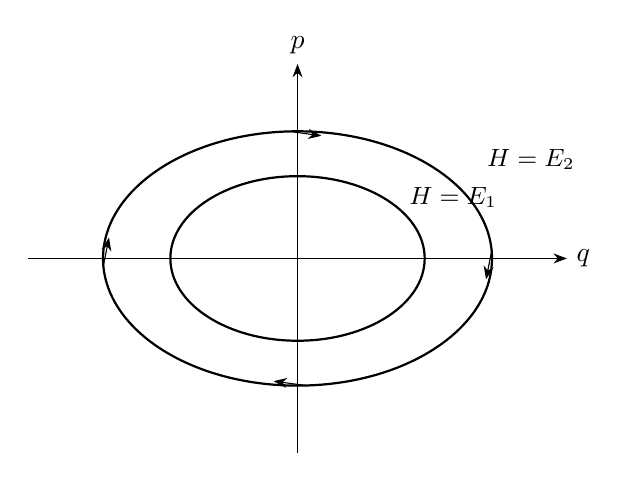
\begin{tikzpicture}[>=Stealth, scale=0.95]
  \draw[->] (-3.6,0) -- (3.6,0) node[right] {$q$};
  \draw[->] (0,-2.6) -- (0,2.6) node[above] {$p$};
  \draw[thick] (0,0) ellipse (2.6cm and 1.7cm);
  \draw[thick] (0,0) ellipse (1.7cm and 1.1cm);
  \draw[->] (2.6,0.12) -- (2.52,-0.28);
  \draw[->] (0.12,-1.7) -- (-0.32,-1.64);
  \draw[->] (-2.6,-0.12) -- (-2.52,0.28);
  \draw[->] (-0.12,1.7) -- (0.32,1.64);
  \node at (3.12,1.32) {\small $H=E_2$};
  \node at (2.08,0.82) {\small $H=E_1$};
\end{tikzpicture}
\caption{Phase space of the harmonic oscillator. Curves of constant $H$ are ellipses. Arrows are the Hamiltonian flow, clockwise. A larger ellipse is a larger energy. The flow never crosses ellipses because $\dot H=0$.}
\end{figure}

\subsection{Forbidden laws}

Hamilton's equations automatically give a deterministic reversible flow: one vector $(\qdot,\pdot)$ at each phase-space point. For standard $H(q,p)$ with $H$ even in $p$, reversing $p\to -p$ and $t\to -t$ runs the trajectory backward.

A law that made all trajectories fall into a sink would not come from any $H$. In one degree of freedom, $\qdot=\partial H/\partial p$ and $\pdot=-\partial H/\partial q$ imply
\[
\pd{\qdot}{q}+\pd{\pdot}{p}=0
\]
identically (Lecture~7). A sink has negative divergence. Friction, and any rule that shrinks a blob of states onto a point, is excluded. You can still write a differential equation for a damped oscillator. You cannot write it as Hamilton's equations on that $(q,p)$.

The minus-first law, at this stage, is the statement that the arrows on phase space come from an $H$ and therefore do not converge.

%----------------------------------------------------------------------
\section{Lecture 7. Liouville's theorem}

Watch not one system but a cloud of systems, a little region of phase space. Each point moves by Hamilton's equations. Liouville's theorem: the volume of the region is constant in time. Hamiltonian flow is incompressible. That is the continuum version of conservation of information: states are not created or destroyed, and they are not packed into a smaller volume. Poisson brackets then package the same flow as a derivative: $\dot F=\{F,H\}$.

\subsection{Energy surfaces}

Because $\dot H=0$, a single trajectory stays on $H(q,p)=E$. A cloud of systems with a spread of energies occupies a thickened shell around one surface; a cloud of systems with exactly the same $E$ lives on the surface. The cloud can stretch and fold. It cannot shrink to a point, and it cannot leave its energy shell.

In one degree of freedom the ``surface'' is a curve and the motion is determined by $E$ up to a discrete choice of direction. In more degrees of freedom the flow on $H=E$ can be complicated. Liouville still applies to the full $2n$-dimensional volume, and also to the induced volume on the energy surface.

\subsection{Flow and divergence}

Write $\vect{u}=(\qdot,\pdot)$ for the velocity of the flow in $(q,p)$. For one degree of freedom
\[
\vect{u} = \Bigl(\pd{H}{p},\,-\pd{H}{q}\Bigr).
\]
The divergence is
\begin{equation}
\label{eq:divu}
\nabla\cdot\vect{u}
= \pd{}{q}\Bigl(\pd{H}{p}\Bigr) + \pd{}{p}\Bigl(-\pd{H}{q}\Bigr)
= \frac{\partial^2 H}{\partial q\,\partial p} - \frac{\partial^2 H}{\partial p\,\partial q}
= 0.
\end{equation}
In $n$ degrees of freedom the same cancellation happens pair by pair:
\[
\sum_{i=1}^n\Biggl(
\pd{}{q_i}\pd{H}{p_i} + \pd{}{p_i}\Bigl(-\pd{H}{q_i}\Bigr)
\Biggr) = 0.
\]
A vector field with vanishing divergence is incompressible. The continuity equation for a density $\rho(q,p,t)$ of systems,
\[
\pd{\rho}{t} + \nabla\cdot(\rho\vect{u}) = 0,
\]
reduces to $\mathrm{D}\rho/\mathrm{D}t=0$ along the flow when $\nabla\cdot\vect{u}=0$: the density following a trajectory is constant. Volume of any comoving region is therefore constant.

A cube of sides $\Delta q$, $\Delta p$ may get long and thin. The product $\Delta q\,\Delta p$ (the area, in one degree of freedom) stays the same.

\subsection{Toy Hamiltonian: shear}

The mechanism is visible for a free particle, $H=p^2/(2m)$. Then $\qdot=p/m$, $\pdot=0$. Points do not move in the $p$ direction. They drift in $q$ at a speed proportional to $p$. A rectangle shears into a parallelogram: the top edge (larger $p$) outruns the bottom. Base times height is constant, so area is constant. Nothing rotates back; the blob just gets more slanted. That is Liouville without curvature of the energy surface.

\begin{figure}[ht]
\centering
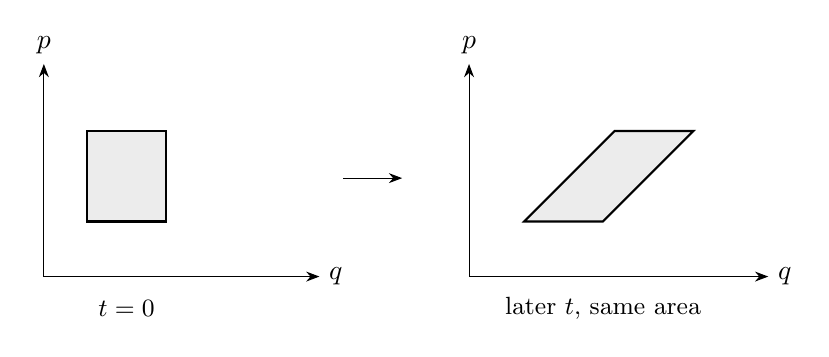
\begin{tikzpicture}[>=Stealth]
  \draw[->] (0,0) -- (3.5,0) node[right] {$q$};
  \draw[->] (0,0) -- (0,2.7) node[above] {$p$};
  \draw[thick, fill=gray!15] (0.55,0.7) rectangle (1.55,1.85);
  \node at (1.05,-0.4) {\small $t=0$};

  \draw[->] (3.8,1.25) -- (4.55,1.25);

  \begin{scope}[xshift=5.4cm]
    \draw[->] (0,0) -- (3.8,0) node[right] {$q$};
    \draw[->] (0,0) -- (0,2.7) node[above] {$p$};
    \draw[thick, fill=gray!15]
      (0.7,0.7) -- (1.7,0.7) -- (2.85,1.85) -- (1.85,1.85) -- cycle;
    \node at (1.7,-0.4) {\small later $t$, same area};
  \end{scope}
\end{tikzpicture}
\caption{Liouville, shown as free-particle shear. $\qdot=p/m$, $\pdot=0$: larger $p$ runs ahead in $q$. The rectangle becomes a parallelogram of the same area. A damped oscillator would shrink the region; that flow is not Hamiltonian.}
\end{figure}

For a generic $H$ the blob also stretches along energy surfaces and folds. The local Jacobian determinant of the flow map remains $1$. Topology of a small patch: it can be deformed arbitrarily (subject to volume) but not crushed.

\subsection{Counterexample: damping}

The damped oscillator
\[
\ddot q + \gamma\qdot + \omega^2 q = 0
\]
with $p=m\qdot$ gives the phase-space field
\[
\qdot = \frac{p}{m},\qquad
\pdot = -m\omega^2 q - \gamma p.
\]
Divergence:
\[
\nabla\cdot\vect{u} = 0 + (-\gamma) = -\gamma.
\]
Areas shrink as $e^{-\gamma t}$. Trajectories spiral into the origin. There is no $H(q,p)$ whose Hamilton equations produce this $\vect{u}$, because every Hamiltonian field has $\nabla\cdot\vect{u}=0$.

Friction is a bookkeeping device for degrees of freedom you have chosen not to track (microscopic motion in the damper, heat). The full isolated system still obeys Liouville in a larger phase space. The reduced description on $(q,p)$ does not.

\subsection{Poisson brackets}

For two functions $F(q,p)$, $G(q,p)$,
\begin{equation}
\label{eq:PB}
\{F,G\} = \pd{F}{q}\pd{G}{p} - \pd{F}{p}\pd{G}{q}.
\end{equation}
In $n$ dimensions, sum over $i$:
\[
\{F,G\} = \sum_i\Biggl(
\pd{F}{q_i}\pd{G}{p_i} - \pd{F}{p_i}\pd{G}{q_i}
\Biggr).
\]
Hamilton's equations become
\[
\qdot = \{q,H\},\qquad \pdot = \{p,H\}.
\]
For any $F(q,p,t)$,
\begin{equation}
\label{eq:Fdot}
\ddt F = \{F,H\} + \pd{F}{t}.
\end{equation}
Derivation: along a trajectory,
\[
\dot F = \pd{F}{q}\qdot + \pd{F}{p}\pdot + \pd{F}{t}
= \pd{F}{q}\pd{H}{p} + \pd{F}{p}\Bigl(-\pd{H}{q}\Bigr) + \pd{F}{t}.
\]
If $F$ has no explicit time dependence, $\dot F=\{F,H\}$. Conserved quantities are those with $\{F,H\}=0$.

Basic brackets, from the definition:
\[
\{q,p\}=1,\qquad \{q,q\}=0,\qquad \{p,p\}=0,
\]
and $\{q_i,p_j\}=\delta_{ij}$ in several dimensions.

The Poisson bracket is the object that turns ``$H$ generates time evolution'' into a formula that works for every observable at once. Next lecture it also generates translations and rotations.

%----------------------------------------------------------------------
\section{Lecture 8. Poisson brackets}

The Poisson bracket is an algebra on functions of phase space: antisymmetric, Leibniz, Jacobi. Time evolution is $\dot F=\{F,H\}$. An infinitesimal symmetry generated by a charge $Q$ is $\delta F=\varepsilon\{F,Q\}$. Conservation of $Q$ is $\{Q,H\}=0$, which is the same equation as ``$Q$ generates a symmetry of $H$.'' That is Noether in this language. The first nontrivial algebra is $\{L_i,L_j\}=\varepsilon_{ijk}L_k$. Once you have it, rigid-body motion follows from $H(L)$ without returning to the original angles.

\subsection{The algebra}

From the definition,
\begin{align}
\{F,G\} &= -\{G,F\}, \label{eq:PBanti}\\
\{F,aG+bK\} &= a\{F,G\}+b\{F,K\}, \nonumber\\
\{F,GK\} &= \{F,G\}K + G\{F,K\}, \label{eq:PBleibniz}\\
\{F,\{G,K\}\} + \{G,\{K,F\}\} + \{K,\{F,G\}\} &= 0. \label{eq:PBjacobi}
\end{align}
Antisymmetry and linearity are obvious. Leibniz is the product rule for derivatives. The Jacobi identity is a short grind in components; the content is that $\{F,\,\cdot\,\}$ acts as a derivation of the bracket itself.

This is the same algebra that commutators satisfy in quantum mechanics, with the replacement $\{,\}\leftrightarrow [\, ,\,]/i\hbar$. That is why the course leans on Poisson brackets rather than treating them as notation for Hamilton's equations.

A consequence of Jacobi (Poisson's theorem): if $F$ and $G$ both Poisson-commute with $H$, then so does $\{F,G\}$. The bracket of two conserved quantities is conserved. Sometimes it is a new charge, sometimes it is a combination of the ones you had (or zero).

\subsection{Generators of symmetries}

An infinitesimal canonical transformation generated by $Q(q,p)$ is
\[
\delta F = \varepsilon\{F,Q\}
\]
for every $F$. In particular
\[
\delta q = \varepsilon\{q,Q\} = \varepsilon\pd{Q}{p},\qquad
\delta p = \varepsilon\{p,Q\} = -\varepsilon\pd{Q}{q}.
\]

\textbf{Translations.} Take $Q=p$. Then $\{q,p\}=1$, $\{p,p\}=0$, so $\delta q=\varepsilon$, $\delta p=0$. Momentum generates translations in $q$.

\textbf{Time evolution.} Take $Q=H$ and $\varepsilon=dt$. Then $\delta F=dt\,\{F,H\}=\dot F\,dt$. The Hamiltonian generates time translations along the flow.

\textbf{Rotations.} Take $Q=L_z=x p_y-y p_x$. Then
\begin{align*}
\{x,L_z\} &= \{x, x p_y - y p_x\} = -y\{x,p_x\} = -y,\\
\{y,L_z\} &= \{y, x p_y - y p_x\} = x\{y,p_y\} = x,\\
\{p_x,L_z\} &= -p_y,\qquad \{p_y,L_z\}=p_x.
\end{align*}
So $\delta x=-\varepsilon y$, $\delta y=\varepsilon x$, and $\vect{p}$ rotates the same way. $L_z$ generates rotations about $z$.

If $Q$ generates a symmetry of the dynamics, the transformation leaves $H$ invariant: $\delta H=\varepsilon\{H,Q\}=0$, hence $\{Q,H\}=0$, hence $\dot Q=0$. Conversely, a conserved $Q$ generates a transformation that leaves $H$ invariant. Conservation and symmetry are the same equation, $\{Q,H\}=0$.

\subsection{Angular momentum algebra}

For $\vect{L}=\vect{r}\times\vect{p}$,
\[
L_x = y p_z - z p_y,\qquad
L_y = z p_x - x p_z,\qquad
L_z = x p_y - y p_x.
\]
Compute $\{L_x,L_y\}$. Expand and use $\{y,p_y\}=1$, $\{z,p_z\}=1$, and that distinct Cartesian pairs bracket to zero:
\begin{align*}
\{L_x,L_y\}
&= \{y p_z - z p_y,\, z p_x - x p_z\}\\
&= \{y p_z,\, z p_x\} - \{y p_z,\, x p_z\}
- \{z p_y,\, z p_x\} + \{z p_y,\, x p_z\}.
\end{align*}
The middle two brackets vanish. The first is
\[
\{y p_z,\, z p_x\} = y\{p_z,z\}p_x = -y p_x,
\]
and the last is
\[
\{z p_y,\, x p_z\} = p_y x\{z,p_z\} = x p_y.
\]
So
\[
\{L_x,L_y\} = -y p_x + x p_y = L_z.
\]
Cycling indices,
\begin{equation}
\label{eq:Lalg}
\{L_i,L_j\} = \varepsilon_{ijk} L_k.
\end{equation}
Also $\{L_i,L^2\}=0$ by Leibniz and antisymmetry: $L^2$ is a scalar, and each $L_i$ generates rotations, which do not change $L^2$.

If $H$ is rotationally invariant, $\{L_i,H\}=0$, so each component of $\vect{L}$ is conserved. You cannot always specify all three as labels of a trajectory in a naive way, because they do not Poisson-commute with each other. You can specify $L_z$ and $L^2$. That pattern survives in quantum mechanics as $[L_i,L_j]=i\hbar\varepsilon_{ijk}L_k$ and simultaneous eigenstates of $L^2$ and $L_z$.

\subsection{Gyroscope}

A rigid body, principal axes, inertia $I_1,I_2,I_3$. Kinetic energy is quadratic in the body-frame angular velocity, or equivalently
\[
H = \frac{L_1^2}{2I_1} + \frac{L_2^2}{2I_2} + \frac{L_3^2}{2I_3}
\]
in terms of the body-frame components of angular momentum. The Poisson structure on those components is the rigid-body one, $\{L_i,L_j\}=-\varepsilon_{ijk}L_k$ (the minus relative to \eqref{eq:Lalg} is the body-frame convention). Then
\[
\dot L_i = \{L_i,H\}
\]
produces Euler's equations. Explicitly, $\partial H/\partial L_j=L_j/I_j=\omega_j$, and
\[
\dot L_1 = -\bigl(\omega_2 L_3 - \omega_3 L_2\bigr) = (I_2-I_3)\omega_2\omega_3,
\]
and cyclic, or
\[
I_1\dot\omega_1 - (I_2-I_3)\omega_2\omega_3 = 0,
\]
and cyclic. Torque-free motion of $\vect{\omega}$ in the body follows from $H(L)$ and the algebra. You do not go back to Euler angles.

The spherical case $I_1=I_2=I_3$ has $H\propto L^2$, so $\dot{\vect{L}}=0$ in this algebra, as it must. The asymmetric top is the first place the nonlinear Euler equations show up, and they showed up without a Lagrangian in $\theta,\phi,\psi$.

That is the point of the algebra: once you know $\{L_i,L_j\}$ and $H(L)$, the motion of $\vect{L}$ is determined.

%----------------------------------------------------------------------
\section{Lecture 9. Electric and magnetic fields, part 1}

The Lorentz force $q(\vect{E}+\vect{v}\times\vect{B})$ is not $-\nabla V(\vect{r})$. The magnetic piece depends on velocity and is perpendicular to $\vect{v}$, so it does no work. To put this force into an action principle you need a term in $L$ linear in velocity. The term that works is $q\,\vect{v}\cdot\vect{A}$, where $\vect{B}=\nabla\times\vect{A}$. The vector potential is needed because the action is a scalar built from positions and velocities; $\vect{B}$ itself is not that kind of object. Gauge freedom is the leftover ambiguity in $\vect{A}$ at fixed $\vect{B}$.

\subsection{Fields}

At each point of space there is an electric field $\vect{E}(\vect{r})$ and a magnetic field $\vect{B}(\vect{r})$. This course treats them as given background, static for Lectures~9 and~10. A field is an assignment of a vector (or a scalar) to each $\vect{r}$, not a mechanical degree of freedom being varied here. (Maxwell's equations, which make $\vect{E}$ and $\vect{B}$ dynamical, are a later course.)

A charge $q$ feels the Lorentz force
\begin{equation}
\label{eq:Lorentz}
\vect{F} = q\bigl(\vect{E} + \vect{v}\times\vect{B}\bigr).
\end{equation}
The magnetic piece is perpendicular to $\vect{v}$:
\[
\vect{v}\cdot(\vect{v}\times\vect{B}) = 0,
\]
so it does no work. It changes direction, not speed. Kinetic energy $\tfrac12 m v^2$ is unaffected by $\vect{B}$ alone. A static $\vect{E}$ does work; that part comes from a potential $\Phi$.

\subsection{Nabla, gradient, divergence, curl}

The operator $\nabla$ is the vector of derivatives $(\partial_x,\partial_y,\partial_z)$. On a scalar $\Phi$ and a vector $\vect{A}$,
\begin{align*}
\operatorname{grad}\Phi &= \nabla\Phi,\\
\operatorname{div}\vect{A} &= \nabla\cdot\vect{A},\\
\operatorname{curl}\vect{A} &= \nabla\times\vect{A}.
\end{align*}
In components,
\[
(\nabla\Phi)_i = \partial_i\Phi,\qquad
\nabla\cdot\vect{A} = \partial_i A_i,\qquad
(\nabla\times\vect{A})_i = \epsijk\partial_j A_k,
\]
with summation over repeated indices.

The gradient points toward increasing $\Phi$; its magnitude is the slope. The divergence at a point is the net flux of $\vect{A}$ out of a small volume, per unit volume. The curl measures local rotation of the vector field (circulation around a small loop, per unit area).

\subsection{Levi-Civita and the two identities}

The Levi-Civita symbol $\epsijk$ is totally antisymmetric, with $\varepsilon_{123}=1$. Then $(\vect{a}\times\vect{b})_i=\epsijk a_j b_k$. The contraction identity
\[
\epsijk\varepsilon_{ilm} = \delta_{jl}\delta_{km}-\delta_{jm}\delta_{kl}
\]
turns products of two $\varepsilon$'s into Kronecker deltas.

Two identities used constantly:
\begin{equation}
\label{eq:vecid}
\nabla\times(\nabla\Phi)=0,\qquad
\nabla\cdot(\nabla\times\vect{A})=0.
\end{equation}
Proof: $(\nabla\times\nabla\Phi)_i=\epsijk\partial_j\partial_k\Phi$. The pair $\partial_j\partial_k$ is symmetric in $jk$, $\epsijk$ is antisymmetric, so the contraction is zero. Similarly $\nabla\cdot(\nabla\times\vect{A})=\epsijk\partial_i\partial_j A_k=0$ by antisymmetry in $ij$.

These are why potentials exist. If $\nabla\times\vect{E}=0$ (electrostatics, or Faraday with static $\vect{B}$), then locally $\vect{E}=-\nabla\Phi$. If $\nabla\cdot\vect{B}=0$, then locally $\vect{B}=\nabla\times\vect{A}$.

\subsection{Vector potential}

In the Maxwell theory there are no magnetic monopoles, $\nabla\cdot\vect{B}=0$. Then one can write
\begin{equation}
\label{eq:BcurlA}
\vect{B} = \nabla\times\vect{A}
\end{equation}
for a vector potential $\vect{A}$. For static electric fields, $\nabla\times\vect{E}=0$ and
\[
\vect{E} = -\nabla\Phi.
\]
(Time-dependent fields add $\vect{E}=-\nabla\Phi-\partial\vect{A}/\partial t$. This course stays static.)

Why introduce $\vect{A}$ if $\vect{B}$ is the measurable field? Because the action is $\int L\,dt$ with $L$ a scalar function of $\vect{r}$ and $\vect{v}$. You can couple to $\Phi$ by $-q\Phi$. You cannot couple to $\vect{B}$ by a term $q\vect{r}\cdot\vect{B}$ or similar and get $\vect{v}\times\vect{B}$ out of Euler-Lagrange. You \emph{can} couple to $\vect{A}$ by $q\vect{v}\cdot\vect{A}$, which is a scalar, linear in $\vect{v}$, and (as Lecture~10 computes) produces $q\vect{v}\times(\nabla\times\vect{A})$. The vector potential is the object the least-action principle can eat. $\vect{B}$ is then $\nabla\times\vect{A}$ by definition in this setup.

\subsection{Gauge}

$\vect{A}$ is not unique. If $\vect{A}$ works, so does
\begin{equation}
\label{eq:gauge}
\vect{A}\to\vect{A}+\nabla\lambda
\end{equation}
for any scalar $\lambda(\vect{r})$, because $\nabla\times\nabla\lambda=0$. For static fields one may keep $\Phi$ fixed, or (in the time-dependent theory) send $\Phi\to\Phi-\partial\lambda/\partial t$ at the same time. Physics depends on $\vect{E}$ and $\vect{B}$, not on a particular choice of $\vect{A}$. Equations of motion must be gauge invariant. $L$ itself need not be; it may change by a total time derivative.

``Gauge'' here is this redundancy in the potential, not a measuring instrument. Different gauges are different $\vect{A}$'s with the same curl. Some gauges make a coordinate cyclic and the problem integrable (Lecture~10). The orbit does not care which gauge you used.

\subsection{Lagrangian for a charge}

Ordinary $L=T-V$ produces $\vect{F}=-\nabla V$, independent of velocity. The magnetic force is not of that form. You need a term linear in velocity. The Lagrangian that reproduces \eqref{eq:Lorentz} is
\begin{equation}
\label{eq:LEM}
L = \tfrac12 m \vect{v}^2 - q\Phi(\vect{r}) + q\,\vect{v}\cdot\vect{A}(\vect{r}).
\end{equation}
The last term is the same kind of object as the Coriolis term $m\vect{v}\cdot(\vect{\omega}\times\vect{r})$ in a rotating frame. Both are $\vect{v}$ dotted into a vector built from the configuration. Both produce a force $\propto\vect{v}\times(\mathrm{curl}\text{ of that vector})$. For Coriolis, $\mathrm{curl}(\vect{\omega}\times\vect{r})=2\vect{\omega}$ if $\vect{\omega}$ is constant. For magnetism, $\mathrm{curl}\,\vect{A}=\vect{B}$. The analogy is structural: same slot in $L$, same kind of force. It is not an identification of $\vect{B}$ with $2\vect{\omega}$.

The electric piece $-q\Phi$ is an ordinary potential. The magnetic piece cannot be absorbed into $\Phi$.

\subsection{Gauge invariance of the equations of motion}

Under $\vect{A}\to\vect{A}+\nabla\lambda$, with $\Phi$ fixed (static),
\[
L \to L + q\,\vect{v}\cdot\nabla\lambda.
\]
Along the trajectory, $\vect{v}\cdot\nabla\lambda=\dot\lambda(\vect{r}(t))$, so
\[
L \to L + q\,\ddt\lambda\bigl(\vect{r}(t)\bigr).
\]
The extra piece is a total time derivative. The action changes by $q\bigl[\lambda(t_2)-\lambda(t_1)\bigr]$, which does not affect Euler-Lagrange when the endpoints are fixed. The equations of motion are gauge invariant even though $L$ is not.

That is the same loophole as $L\to L+\dot F$ in Lecture~3. Gauge transformations are a physical family of such additions, labeled by $\lambda(\vect{r})$.

The explicit check that Euler-Lagrange on \eqref{eq:LEM} is the Lorentz force is Lecture~10. The reason to believe it already: the only gauge-invariant, rotationally scalar, linear-in-$\vect{v}$ coupling built from $\vect{A}$ is $\vect{v}\cdot\vect{A}$, and it has to be there if magnetism is to come from an action.

%----------------------------------------------------------------------
\section{Lecture 10. Electric and magnetic fields, part 2}

Everything in the course is on the table at once: $L$, gauge, cyclic coordinates, canonical momentum, $H$, Euler-Lagrange, conservation laws. A particle in a static $\vect{B}$ is the example that uses all of them. The distinction that must not be blurred: Noether conserves \emph{canonical} momentum $p=\partial L/\partial v$, which is $m\vect{v}+q\vect{A}$, not the mechanical $m\vect{v}$. Gauge choice can make a coordinate cyclic; then a component of $\vect{p}$ is conserved and the cyclotron orbit falls out.

\subsection{Canonical versus mechanical momentum}

From \eqref{eq:LEM},
\begin{equation}
\label{eq:pcan}
p_i = \pd{L}{v_i} = m v_i + q A_i,
\end{equation}
or $\vect{p}=m\vect{v}+q\vect{A}$. The \emph{mechanical} momentum is $m\vect{v}=\vect{p}-q\vect{A}$. The \emph{canonical} momentum is $\vect{p}$.

Noether conserves canonical momenta when the corresponding coordinates are cyclic. In a magnetic field, $m\vect{v}$ is generally not conserved even if the physics is translation invariant in some gauge. Under a gauge transformation, $\vect{A}$ changes by $\nabla\lambda$, so $\vect{p}$ changes by $q\nabla\lambda$. Mechanical $\vect{v}$ is gauge invariant (it is $d\vect{r}/dt$). Canonical $\vect{p}$ is not. Conservation laws are statements about $\vect{p}$ in a given gauge, not about $m\vect{v}$.

This is the same phenomenon as polar $p_\theta=m r^2\dot\theta\neq m\dot\theta$. The conjugate momentum is whatever $\partial L/\partial\qdot$ is, and that is the Noether charge.

\subsection{Hamiltonian}

Legendre transform, $\vect{v}=(\vect{p}-q\vect{A})/m$:
\begin{align*}
H
&= \vect{p}\cdot\vect{v}-L
= \vect{p}\cdot\vect{v} - \tfrac12 m v^2 + q\Phi - q\vect{v}\cdot\vect{A}.
\end{align*}
Substitute $\vect{p}=m\vect{v}+q\vect{A}$, so $\vect{p}\cdot\vect{v}=m v^2+q\vect{v}\cdot\vect{A}$:
\[
H = m v^2 + q\vect{v}\cdot\vect{A} - \tfrac12 m v^2 + q\Phi - q\vect{v}\cdot\vect{A}
= \tfrac12 m v^2 + q\Phi.
\]
In canonical variables,
\begin{equation}
\label{eq:HEM}
H = \frac{(\vect{p}-q\vect{A})^2}{2m} + q\Phi.
\end{equation}
$H$ is mechanical kinetic energy plus $q\Phi$. It is not $\vect{p}^2/2m+q\Phi$. The combination $\vect{p}-q\vect{A}$ is gauge invariant, and so is $H$. Hamilton's equations from \eqref{eq:HEM} are the Lorentz force law. The $\vect{A}$ dependence in $H$ is how magnetism sits in Hamiltonian mechanics: it shifts the momentum that kinetic energy is quadratic in.

\subsection{Euler-Lagrange recovers Lorentz}

Compute from \eqref{eq:LEM}, static $\Phi$ and $\vect{A}$. The $x$-equation is representative.
\[
\pd{L}{\dot x} = m\dot x + q A_x,
\]
\[
\ddt\pd{L}{\dot x}
= m\ddot x + q\bigl(\dot x\,\partial_x A_x + \dot y\,\partial_y A_x + \dot z\,\partial_z A_x\bigr)
= m\ddot x + q\,(\vect{v}\cdot\nabla)A_x.
\]
\[
\pd{L}{x} = -q\,\partial_x\Phi + q\,\vect{v}\cdot\partial_x\vect{A}.
\]
Euler-Lagrange:
\[
m\ddot x + q\,(\vect{v}\cdot\nabla)A_x
= -q\,\partial_x\Phi + q\,\vect{v}\cdot\partial_x\vect{A},
\]
\[
m\ddot x
= -q\,\partial_x\Phi
+ q\Bigl(\vect{v}\cdot\partial_x\vect{A} - (\vect{v}\cdot\nabla)A_x\Bigr).
\]
The parenthesis is the $x$-component of $\vect{v}\times(\nabla\times\vect{A})$. Check:
\begin{align*}
\bigl[\vect{v}\times(\nabla\times\vect{A})\bigr]_x
&= v_y(\partial_x A_y-\partial_y A_x) - v_z(\partial_z A_x-\partial_x A_z)\\
&= \vect{v}\cdot\partial_x\vect{A} - (\vect{v}\cdot\nabla)A_x,
\end{align*}
the $v_x\partial_x A_x$ terms cancelling in the difference. With $\vect{B}=\nabla\times\vect{A}$ and $\vect{E}=-\nabla\Phi$,
\[
m\dot{\vect{v}} = q\bigl(\vect{E}+\vect{v}\times\vect{B}\bigr).
\]
The vector potential is needed if you want a least-action principle. The force law itself mentions only $\vect{E}$ and $\vect{B}$. After the derivatives act, $\vect{A}$ disappears in favor of its curl.

\subsection{Gauges for a uniform field}

A constant $\vect{B}=B\hat{\vect{z}}$ can be written, among other ways,
\begin{align}
\vect{A}_{\mathrm{sym}}
&= \tfrac12\vect{B}\times\vect{r}
= \bigl(-\tfrac12 B y,\,\tfrac12 B x,\,0\bigr), \label{eq:Asym}\\
\vect{A}_{\mathrm{L}}
&= (-B y,\, 0,\, 0). \label{eq:ALandau}
\end{align}
The first is symmetric gauge, the second is Landau gauge. They differ by a gradient:
\[
\vect{A}_{\mathrm{L}} - \vect{A}_{\mathrm{sym}}
= \bigl(-\tfrac12 B y,\, -\tfrac12 B x,\, 0\bigr)
= \nabla\Bigl(-\tfrac12 B x y\Bigr).
\]
Same $\vect{B}$. In symmetric gauge, $L$ depends on $x$ and $y$ together (rotationally nicer, $p_\theta$ related to $L_z$). In Landau gauge, $L$ does not depend on $x$. That is a smart choice for solving, not a different physical field.

\subsection{Landau gauge, cyclic coordinate, cyclotron motion}

Take $\Phi=0$, $\vect{A}=(-By,0,0)$. Then
\[
L = \tfrac12 m(\dot x^2+\dot y^2+\dot z^2) - q B y\,\dot x.
\]
$x$ is cyclic, so
\[
p_x = m\dot x - q B y
\]
is conserved. $z$ is cyclic, $p_z=m\dot z$ conserved (uniform motion along $\vect{B}$). Energy
\[
H = \frac{1}{2m}\bigl[(p_x + q B y)^2 + p_y^2 + p_z^2\bigr]
\]
is conserved. Mechanical velocities:
\[
m\dot x = p_x + q B y,\qquad m\dot y = p_y,\qquad m\dot z = p_z.
\]
Hamilton's equation for $p_y$, or Euler-Lagrange in $y$, gives
\[
m\ddot y = -q B\dot x = -\frac{q B}{m}(p_x + q B y).
\]
Rearrange:
\[
\ddot y + \omega_c^2 \bigl(y - y_0\bigr) = 0,
\qquad
\omega_c = \frac{q B}{m},\qquad
y_0 = -\frac{p_x}{q B}.
\]
So $y$ oscillates about $y_0$ at the cyclotron frequency $\omega_c$. From $m\dot x=p_x+qBy=qB(y-y_0)$,
\[
\dot x=\omega_c(y-y_0).
\]
If $y-y_0=R\cos(\omega_c t+\phi)$, then $\dot x=\omega_c R\cos(\omega_c t+\phi)$, so $x-x_0=R\sin(\omega_c t+\phi)$. The orbit in the $xy$-plane is a circle of radius
\[
R = \frac{v_\perp}{\omega_c}
\]
centered at a guiding center whose $y$-coordinate is $y_0=-p_x/(qB)$. The conserved $p_x$ labels that center, not the mechanical $m\dot x$. Plus uniform motion along $z$.

You can get the same circle from the Lorentz force $m\vect{a}=q\vect{v}\times\vect{B}$ without ever mentioning $A$: $\ddot x=\omega_c\dot y$, $\ddot y=-\omega_c\dot x$. The Lagrangian route is the one that makes the conserved $p_x$ visible, and that explains why a gauge choice (cyclic $x$) produced a conservation law that locates the guiding center.

\subsection{Monopoles}

If magnetic monopoles existed, $\nabla\cdot\vect{B}\neq 0$ in a region, and \eqref{eq:vecid} would forbid a globally smooth $\vect{A}$ with $\vect{B}=\nabla\times\vect{A}$ on that region. You can still work with $\vect{A}$ on overlapping patches, with a gauge transformation on the overlap (Dirac's construction). A string singularity in $\vect{A}$ (the Dirac string) can be moved by a gauge transformation; requiring that it be unphysical quantizes the product of electric and magnetic charge. The lectures flag this in the questions. They do not build the theory. For everything in Lectures~9 and~10, $\nabla\cdot\vect{B}=0$ and a single $\vect{A}$ is enough.

%----------------------------------------------------------------------
\section*{Formula sheet}

\begin{align*}
F&=ma=\dot p,\quad p=mv \\[0.3em]
L&=T-V,\quad
\ddt\pd{L}{\qdot}=\pd{L}{q},\quad
p=\pd{L}{\qdot} \\[0.3em]
H&=p\qdot-L,\quad
\qdot=\pd{H}{p},\quad
\pdot=-\pd{H}{q},\quad
\dot H=\pd{H}{t} \\[0.3em]
\{F,G\}&=\pd{F}{q}\pd{G}{p}-\pd{F}{p}\pd{G}{q},\quad
\dot F=\{F,H\}+\pd{F}{t} \\[0.3em]
\{q,p\}&=1,\quad \{L_i,L_j\}=\varepsilon_{ijk}L_k \\[0.3em]
\nabla\times\nabla\Phi&=0,\quad \nabla\cdot(\nabla\times A)=0,\quad B=\nabla\times A \\[0.3em]
F&=q(E+v\times B),\quad
L_{\mathrm{EM}}=\tfrac12 mv^2-q\Phi+q v\cdot A \\[0.3em]
p&=mv+qA,\quad
H_{\mathrm{EM}}=\frac{(p-qA)^2}{2m}+q\Phi,\quad
\omega_c=\frac{qB}{m}
\end{align*}

\vspace{0.8em}
\noindent\emph{Noether (continuous symmetry $q\to q+\varepsilon\eta$):} $Q=p\eta$ conserved.
Translation $\eta=1$ gives $P$. Rotation $\eta=(-y,x)$ gives $L_z$. Time translation gives $H$.

\vspace{0.4em}
\noindent\emph{Liouville:} $\nabla\cdot u=0$ for $u=(\partial H/\partial p,-\partial H/\partial q)$. Phase-space volume is conserved.

\vspace{0.4em}
\noindent\emph{Rotating frame:} $m a=-\nabla V-2m\,\omega\times v-m\,\omega\times(\omega\times r)$.

\vspace{1em}
\noindent\emph{Lectures:}
\url{https://theoreticalminimum.com/courses/classical-mechanics/2011/fall}

\end{document}
